\documentclass[]{article}
\usepackage{lmodern}
\usepackage{amssymb,amsmath}
\usepackage{ifxetex,ifluatex}
\usepackage{fixltx2e} % provides \textsubscript
\ifnum 0\ifxetex 1\fi\ifluatex 1\fi=0 % if pdftex
  \usepackage[T1]{fontenc}
  \usepackage[utf8]{inputenc}
\else % if luatex or xelatex
  \ifxetex
    \usepackage{mathspec}
  \else
    \usepackage{fontspec}
  \fi
  \defaultfontfeatures{Ligatures=TeX,Scale=MatchLowercase}
\fi
% use upquote if available, for straight quotes in verbatim environments
\IfFileExists{upquote.sty}{\usepackage{upquote}}{}
% use microtype if available
\IfFileExists{microtype.sty}{%
\usepackage{microtype}
\UseMicrotypeSet[protrusion]{basicmath} % disable protrusion for tt fonts
}{}
\usepackage[margin=1in]{geometry}
\usepackage{hyperref}
\hypersetup{unicode=true,
            pdftitle={sf.chlorodot mini-package},
            pdfauthor={Robert Hickman},
            pdfborder={0 0 0},
            breaklinks=true}
\urlstyle{same}  % don't use monospace font for urls
\usepackage{color}
\usepackage{fancyvrb}
\newcommand{\VerbBar}{|}
\newcommand{\VERB}{\Verb[commandchars=\\\{\}]}
\DefineVerbatimEnvironment{Highlighting}{Verbatim}{commandchars=\\\{\}}
% Add ',fontsize=\small' for more characters per line
\usepackage{framed}
\definecolor{shadecolor}{RGB}{248,248,248}
\newenvironment{Shaded}{\begin{snugshade}}{\end{snugshade}}
\newcommand{\KeywordTok}[1]{\textcolor[rgb]{0.13,0.29,0.53}{\textbf{#1}}}
\newcommand{\DataTypeTok}[1]{\textcolor[rgb]{0.13,0.29,0.53}{#1}}
\newcommand{\DecValTok}[1]{\textcolor[rgb]{0.00,0.00,0.81}{#1}}
\newcommand{\BaseNTok}[1]{\textcolor[rgb]{0.00,0.00,0.81}{#1}}
\newcommand{\FloatTok}[1]{\textcolor[rgb]{0.00,0.00,0.81}{#1}}
\newcommand{\ConstantTok}[1]{\textcolor[rgb]{0.00,0.00,0.00}{#1}}
\newcommand{\CharTok}[1]{\textcolor[rgb]{0.31,0.60,0.02}{#1}}
\newcommand{\SpecialCharTok}[1]{\textcolor[rgb]{0.00,0.00,0.00}{#1}}
\newcommand{\StringTok}[1]{\textcolor[rgb]{0.31,0.60,0.02}{#1}}
\newcommand{\VerbatimStringTok}[1]{\textcolor[rgb]{0.31,0.60,0.02}{#1}}
\newcommand{\SpecialStringTok}[1]{\textcolor[rgb]{0.31,0.60,0.02}{#1}}
\newcommand{\ImportTok}[1]{#1}
\newcommand{\CommentTok}[1]{\textcolor[rgb]{0.56,0.35,0.01}{\textit{#1}}}
\newcommand{\DocumentationTok}[1]{\textcolor[rgb]{0.56,0.35,0.01}{\textbf{\textit{#1}}}}
\newcommand{\AnnotationTok}[1]{\textcolor[rgb]{0.56,0.35,0.01}{\textbf{\textit{#1}}}}
\newcommand{\CommentVarTok}[1]{\textcolor[rgb]{0.56,0.35,0.01}{\textbf{\textit{#1}}}}
\newcommand{\OtherTok}[1]{\textcolor[rgb]{0.56,0.35,0.01}{#1}}
\newcommand{\FunctionTok}[1]{\textcolor[rgb]{0.00,0.00,0.00}{#1}}
\newcommand{\VariableTok}[1]{\textcolor[rgb]{0.00,0.00,0.00}{#1}}
\newcommand{\ControlFlowTok}[1]{\textcolor[rgb]{0.13,0.29,0.53}{\textbf{#1}}}
\newcommand{\OperatorTok}[1]{\textcolor[rgb]{0.81,0.36,0.00}{\textbf{#1}}}
\newcommand{\BuiltInTok}[1]{#1}
\newcommand{\ExtensionTok}[1]{#1}
\newcommand{\PreprocessorTok}[1]{\textcolor[rgb]{0.56,0.35,0.01}{\textit{#1}}}
\newcommand{\AttributeTok}[1]{\textcolor[rgb]{0.77,0.63,0.00}{#1}}
\newcommand{\RegionMarkerTok}[1]{#1}
\newcommand{\InformationTok}[1]{\textcolor[rgb]{0.56,0.35,0.01}{\textbf{\textit{#1}}}}
\newcommand{\WarningTok}[1]{\textcolor[rgb]{0.56,0.35,0.01}{\textbf{\textit{#1}}}}
\newcommand{\AlertTok}[1]{\textcolor[rgb]{0.94,0.16,0.16}{#1}}
\newcommand{\ErrorTok}[1]{\textcolor[rgb]{0.64,0.00,0.00}{\textbf{#1}}}
\newcommand{\NormalTok}[1]{#1}
\usepackage{graphicx,grffile}
\makeatletter
\def\maxwidth{\ifdim\Gin@nat@width>\linewidth\linewidth\else\Gin@nat@width\fi}
\def\maxheight{\ifdim\Gin@nat@height>\textheight\textheight\else\Gin@nat@height\fi}
\makeatother
% Scale images if necessary, so that they will not overflow the page
% margins by default, and it is still possible to overwrite the defaults
% using explicit options in \includegraphics[width, height, ...]{}
\setkeys{Gin}{width=\maxwidth,height=\maxheight,keepaspectratio}
\IfFileExists{parskip.sty}{%
\usepackage{parskip}
}{% else
\setlength{\parindent}{0pt}
\setlength{\parskip}{6pt plus 2pt minus 1pt}
}
\setlength{\emergencystretch}{3em}  % prevent overfull lines
\providecommand{\tightlist}{%
  \setlength{\itemsep}{0pt}\setlength{\parskip}{0pt}}
\setcounter{secnumdepth}{0}
% Redefines (sub)paragraphs to behave more like sections
\ifx\paragraph\undefined\else
\let\oldparagraph\paragraph
\renewcommand{\paragraph}[1]{\oldparagraph{#1}\mbox{}}
\fi
\ifx\subparagraph\undefined\else
\let\oldsubparagraph\subparagraph
\renewcommand{\subparagraph}[1]{\oldsubparagraph{#1}\mbox{}}
\fi

%%% Use protect on footnotes to avoid problems with footnotes in titles
\let\rmarkdownfootnote\footnote%
\def\footnote{\protect\rmarkdownfootnote}

%%% Change title format to be more compact
\usepackage{titling}

% Create subtitle command for use in maketitle
\newcommand{\subtitle}[1]{
  \posttitle{
    \begin{center}\large#1\end{center}
    }
}

\setlength{\droptitle}{-2em}
  \title{sf.chlorodot mini-package}
  \pretitle{\vspace{\droptitle}\centering\huge}
  \posttitle{\par}
  \author{Robert Hickman}
  \preauthor{\centering\large\emph}
  \postauthor{\par}
  \predate{\centering\large\emph}
  \postdate{\par}
  \date{2018-09-09}


\begin{document}
\maketitle

Recently, I'd seen two tweets with stunning examples of maps by Paul
Campbell
\href{https://twitter.com/PaulCampbell91/status/992043182996193280}{here}
and (taken inspiration from the first) by Imer Muhović
\href{https://twitter.com/ImerM1/status/1037358973807210498}{here}.

The basic idea of the dot chloropleths is to visualise not only the
location clustering of each variable but the number of observations
(something traditional `filled' chloropleths don't do). More importantly
than this, the maps also just look really really cool.

I had a spare few minutes during work on Friday which I tidied up into a
package to calculate the random position of dots for such maps which can
be found \href{https://github.com/RobWHickman/sf.chlorodot}{on my
github}.

Below, I'll outline the code for the South African example used in the
package README. Data comes from Adrian Frith's
\href{https://census2011.adrianfrith.com/}{very good 2011 census site}
and \href{https://gadm.org/download_country_v3.html}{gadm} for the
shapefiles.

\begin{Shaded}
\begin{Highlighting}[]
\KeywordTok{library}\NormalTok{(sf)}
\KeywordTok{library}\NormalTok{(ggplot2)}
\KeywordTok{library}\NormalTok{(tidyverse)}
\KeywordTok{library}\NormalTok{(data.table)}
\KeywordTok{library}\NormalTok{(rvest)}

\NormalTok{devtools}\OperatorTok{::}\KeywordTok{install_github}\NormalTok{(}\StringTok{'RobWHickman/sf.chlorodot'}\NormalTok{)}
\KeywordTok{library}\NormalTok{(sf.chlordot)}
\end{Highlighting}
\end{Shaded}

Next, download and scrape the data for the map

\begin{Shaded}
\begin{Highlighting}[]
\CommentTok{#download the South African shapefile fom gadm}
\NormalTok{admin_url <-}\StringTok{ "https://biogeo.ucdavis.edu/data/gadm3.6/Rsf/gadm36_ZAF_3_sf.rds"}
\KeywordTok{download.file}\NormalTok{(admin_url, }\DataTypeTok{destfile =} \StringTok{"shapefiles.rds"}\NormalTok{, }\DataTypeTok{mode =} \StringTok{"wb"}\NormalTok{)}
\NormalTok{south_africa <-}\StringTok{ }\KeywordTok{readRDS}\NormalTok{(}\StringTok{"shapefiles.rds"}\NormalTok{) }\OperatorTok
\StringTok{  }\CommentTok{#convert to sf}
\StringTok{  }\KeywordTok{st_as_sf}\NormalTok{() }\OperatorTok
\StringTok{  }\KeywordTok{select}\NormalTok{(}\DataTypeTok{region =}\NormalTok{ NAME_}\DecValTok{3}\NormalTok{) }\OperatorTok
\StringTok{  }\CommentTok{#merge geometries that have two rows}
\StringTok{  }\KeywordTok{group_by}\NormalTok{(region) }\OperatorTok
\StringTok{  }\KeywordTok{summarise}\NormalTok{()}

\CommentTok{#get the links to the data from Adrian Frith's site}
\NormalTok{sa_data_url <-}\StringTok{ "https://census2011.adrianfrith.com"}
\NormalTok{south_africa_data <-}\StringTok{ }\NormalTok{sa_data_url }\OperatorTok
\StringTok{  }\KeywordTok{read_html}\NormalTok{() }\OperatorTok\StringTok{ }\KeywordTok{html_nodes}\NormalTok{(}\StringTok{".namecell a"}\NormalTok{) }\OperatorTok\StringTok{ }\KeywordTok{html_attr}\NormalTok{(}\StringTok{"href"}\NormalTok{) }\OperatorTok\StringTok{ }\KeywordTok{paste0}\NormalTok{(sa_data_url, .) }\OperatorTok
\StringTok{  }\KeywordTok{lapply}\NormalTok{(., }\ControlFlowTok{function}\NormalTok{(x) }\KeywordTok{read_html}\NormalTok{(x) }\OperatorTok\StringTok{ }\KeywordTok{html_nodes}\NormalTok{(}\StringTok{".namecell a"}\NormalTok{) }\OperatorTok\StringTok{ }\KeywordTok{html_attr}\NormalTok{(}\StringTok{"href"}\NormalTok{) }\OperatorTok\StringTok{ }\KeywordTok{paste0}\NormalTok{(sa_data_url, .)) }\OperatorTok\StringTok{ }\KeywordTok{unlist}\NormalTok{() }\OperatorTok
\StringTok{   }\KeywordTok{lapply}\NormalTok{(., }\ControlFlowTok{function}\NormalTok{(x) }\KeywordTok{read_html}\NormalTok{(x) }\OperatorTok\StringTok{ }\KeywordTok{html_nodes}\NormalTok{(}\StringTok{".namecell a"}\NormalTok{) }\OperatorTok\StringTok{ }\KeywordTok{html_attr}\NormalTok{(}\StringTok{"href"}\NormalTok{) }\OperatorTok\StringTok{ }\KeywordTok{paste0}\NormalTok{(sa_data_url, .)) }\OperatorTok\StringTok{ }\KeywordTok{unlist}\NormalTok{()}

\CommentTok{#scrape the data on primary language from the 2011 South African census}
\NormalTok{language_data <-}\StringTok{ }\KeywordTok{rbindlist}\NormalTok{(}\KeywordTok{lapply}\NormalTok{(south_africa_data, }\ControlFlowTok{function}\NormalTok{(x) \{}
\NormalTok{  read <-}\StringTok{ }\KeywordTok{read_html}\NormalTok{(x)}
\NormalTok{  language_nos <-}\StringTok{ }\NormalTok{read }\OperatorTok\StringTok{ }\KeywordTok{html_nodes}\NormalTok{(}\StringTok{".datacell"}\NormalTok{) }\OperatorTok\StringTok{ }\KeywordTok{html_text}\NormalTok{()}
\NormalTok{  start <-}\StringTok{ }\KeywordTok{grep}\NormalTok{(}\StringTok{"Percentage"}\NormalTok{, language_nos)[}\DecValTok{3}\NormalTok{] }\OperatorTok{+}\StringTok{ }\DecValTok{1}
\NormalTok{  stop <-}\StringTok{ }\KeywordTok{grep}\NormalTok{(}\StringTok{"Population"}\NormalTok{, language_nos) }\OperatorTok{-}\StringTok{ }\DecValTok{1}
  \CommentTok{#some areas have no data}
  \ControlFlowTok{if}\NormalTok{(}\OperatorTok{!}\KeywordTok{is.na}\NormalTok{(start) }\OperatorTok{&}\StringTok{ }\OperatorTok{!}\KeywordTok{is.na}\NormalTok{(stop)) \{}
\NormalTok{    language_nos <-}\StringTok{ }\NormalTok{language_nos[start}\OperatorTok{:}\NormalTok{stop]}
\NormalTok{    language_nos <-}\StringTok{ }\NormalTok{language_nos[}\KeywordTok{seq}\NormalTok{(}\DecValTok{1}\NormalTok{, }\KeywordTok{length}\NormalTok{(language_nos), }\DecValTok{2}\NormalTok{)]}
\NormalTok{  \} }\ControlFlowTok{else}\NormalTok{ \{}
\NormalTok{    language_nos <-}\StringTok{ }\OtherTok{NA}
\NormalTok{  \}}
  
\NormalTok{  languages <-}\StringTok{ }\NormalTok{read }\OperatorTok\StringTok{ }\KeywordTok{html_nodes}\NormalTok{(}\StringTok{"tr > :nth-child(1)"}\NormalTok{) }\OperatorTok\StringTok{ }\KeywordTok{html_text}\NormalTok{()}
\NormalTok{  start <-}\StringTok{ }\KeywordTok{grep}\NormalTok{(}\StringTok{"First language"}\NormalTok{, languages) }\OperatorTok{+}\StringTok{ }\DecValTok{1}
\NormalTok{  stop <-}\StringTok{ }\KeywordTok{grep}\NormalTok{(}\StringTok{"Name"}\NormalTok{, languages) }\OperatorTok{-}\StringTok{ }\DecValTok{1}
  \ControlFlowTok{if}\NormalTok{(}\KeywordTok{length}\NormalTok{(start) }\OperatorTok{>}\StringTok{ }\DecValTok{0} \OperatorTok{&}\StringTok{ }\OperatorTok{!}\KeywordTok{is.na}\NormalTok{(stop)) \{}
\NormalTok{    languages <-}\StringTok{ }\NormalTok{languages[start}\OperatorTok{:}\NormalTok{stop]}
\NormalTok{  \} }\ControlFlowTok{else}\NormalTok{ \{}
\NormalTok{    languages <-}\StringTok{ }\OtherTok{NA}
\NormalTok{  \}}
  
\NormalTok{  region_names <-}\StringTok{ }\NormalTok{read }\OperatorTok\StringTok{ }\KeywordTok{html_nodes}\NormalTok{(}\StringTok{".topname"}\NormalTok{) }\OperatorTok\StringTok{ }\KeywordTok{html_text}\NormalTok{()}
  
  \CommentTok{#combine into a df}
\NormalTok{  df <-}\StringTok{ }\KeywordTok{data.frame}\NormalTok{(}\DataTypeTok{language =}\NormalTok{ languages, }\DataTypeTok{primary_speakers =}\NormalTok{ language_nos, }\DataTypeTok{region =}\NormalTok{ region_names)}
  \KeywordTok{return}\NormalTok{(df)}
\NormalTok{\}))}
\end{Highlighting}
\end{Shaded}

the lanaguage data then needs to be transformed before the dot position
is calculated. It must be in `short' format with variables as column
names. At the same time we can do some cleaning in order to match the
shape areas with the region names from the census and remove data we
don't want to plot

\begin{Shaded}
\begin{Highlighting}[]
\NormalTok{language_data }\OperatorTok
\StringTok{  }\CommentTok{#convert number of speakers to numeric}
\StringTok{  }\KeywordTok{mutate}\NormalTok{(}\DataTypeTok{primary_speakers =} \KeywordTok{as.numeric}\NormalTok{(}\KeywordTok{as.character}\NormalTok{(primary_speakers))) }\OperatorTok
\StringTok{  }\CommentTok{#matching of area names with South African shapefile}
\StringTok{  }\KeywordTok{mutate}\NormalTok{(}\DataTypeTok{region =} \KeywordTok{gsub}\NormalTok{(}\StringTok{" NU"}\NormalTok{, }\StringTok{""}\NormalTok{, region)) }\OperatorTok
\StringTok{  }\KeywordTok{mutate}\NormalTok{(}\DataTypeTok{region =} \KeywordTok{gsub}\NormalTok{(}\StringTok{"Tshwane"}\NormalTok{, }\StringTok{"City of Tshwane"}\NormalTok{, region)) }\OperatorTok
\StringTok{  }\CommentTok{#filter only the data we want to merge}
\StringTok{  }\KeywordTok{filter}\NormalTok{(region }\OperatorTok\StringTok{ }\NormalTok{south_africa}\OperatorTok{$}\NormalTok{region) }\OperatorTok
\StringTok{  }\KeywordTok{filter}\NormalTok{(}\OperatorTok{!}\KeywordTok{is.na}\NormalTok{(language)) }\OperatorTok
\StringTok{  }\KeywordTok{filter}\NormalTok{(language }\OperatorTok{!=}\StringTok{ "Not applicable"}\NormalTok{) }\OperatorTok
\StringTok{  }\CommentTok{#spread the data}
\StringTok{  }\KeywordTok{dcast}\NormalTok{(., region }\OperatorTok{~}\StringTok{ }\NormalTok{language, }\DataTypeTok{value.var =} \StringTok{"primary_speakers"}\NormalTok{, }\DataTypeTok{fun.aggregate =}\NormalTok{ sum) }\OperatorTok
\StringTok{  }\CommentTok{#join in the spatial geometry}
\StringTok{  }\KeywordTok{left_join}\NormalTok{(., south_africa) }\OperatorTok
\StringTok{  }\CommentTok{#convert to sf}
\StringTok{  }\KeywordTok{st_as_sf}\NormalTok{()}
\end{Highlighting}
\end{Shaded}

then we can calculate the random dot position using calc\_dots() from
the sf.chlorodot package. This takes three arguments. The first is the
df to take the data from (language\_data). The second is which variables
to calculate positions for. The easiest way to do this is to use
names(df) and select from there, though a character vector can also be
passed. Finally, n\_per\_dot is the number of observations (speakers of
language x) for each dot on the map. This will affect the look of the
map, but also the processing time (lower n\_per\_dot = greater time) so
play around with it a bit.

\begin{Shaded}
\begin{Highlighting}[]
\CommentTok{#calculate the dot positions using calc_dots from the sf.chlorodot package}
\NormalTok{sf_dots <-}\StringTok{ }\KeywordTok{calc_dots}\NormalTok{(}\DataTypeTok{df =}\NormalTok{ language_data, }\DataTypeTok{col_names =} \KeywordTok{names}\NormalTok{(language_data)[}\DecValTok{2}\OperatorTok{:}\DecValTok{14}\NormalTok{], }\DataTypeTok{n_per_dot =} \DecValTok{1000}\NormalTok{)}
\end{Highlighting}
\end{Shaded}

Finally, we can plot the output of this

\begin{Shaded}
\begin{Highlighting}[]
\CommentTok{#stolen the background colour scheme from Paul Campbell's blog}
\CommentTok{#original inspiration for this package}
\NormalTok{p <-}\StringTok{ }\KeywordTok{ggplot}\NormalTok{() }\OperatorTok{+}
\StringTok{  }\KeywordTok{geom_sf}\NormalTok{(}\DataTypeTok{data =}\NormalTok{ south_africa, }\DataTypeTok{fill =} \StringTok{"transparent"}\NormalTok{,}\DataTypeTok{colour =} \StringTok{"white"}\NormalTok{) }\OperatorTok{+}
\StringTok{  }\KeywordTok{geom_point}\NormalTok{(}\DataTypeTok{data =}\NormalTok{ sf_dots, }\KeywordTok{aes}\NormalTok{(lon, lat, }\DataTypeTok{colour =}\NormalTok{ variable), }\DataTypeTok{size =} \FloatTok{0.1}\NormalTok{) }\OperatorTok{+}
\StringTok{  }\KeywordTok{scale_colour_discrete}\NormalTok{(}\DataTypeTok{name =} \StringTok{"Primary Language"}\NormalTok{) }\OperatorTok{+}
\StringTok{  }\KeywordTok{ggtitle}\NormalTok{(}\StringTok{"Language Diversity in South Africa"}\NormalTok{) }\OperatorTok{+}
\StringTok{  }\KeywordTok{theme_void}\NormalTok{() }\OperatorTok{+}
\StringTok{  }\KeywordTok{guides}\NormalTok{(}\DataTypeTok{colour =} \KeywordTok{guide_legend}\NormalTok{(}\DataTypeTok{override.aes =} \KeywordTok{list}\NormalTok{(}\DataTypeTok{size =} \DecValTok{10}\NormalTok{))) }\OperatorTok{+}
\StringTok{  }\KeywordTok{theme}\NormalTok{(}\DataTypeTok{plot.background =} \KeywordTok{element_rect}\NormalTok{(}\DataTypeTok{fill =} \StringTok{"#212121"}\NormalTok{, }\DataTypeTok{color =} \OtherTok{NA}\NormalTok{), }
        \DataTypeTok{panel.background =} \KeywordTok{element_rect}\NormalTok{(}\DataTypeTok{fill =} \StringTok{"#212121"}\NormalTok{, }\DataTypeTok{color =} \OtherTok{NA}\NormalTok{),}
        \DataTypeTok{legend.background =} \KeywordTok{element_rect}\NormalTok{(}\DataTypeTok{fill =} \StringTok{"#212121"}\NormalTok{, }\DataTypeTok{color =} \OtherTok{NA}\NormalTok{),}
        \DataTypeTok{text =}  \KeywordTok{element_text}\NormalTok{(}\DataTypeTok{color =} \StringTok{"white"}\NormalTok{),}
        \DataTypeTok{title =}  \KeywordTok{element_text}\NormalTok{(}\DataTypeTok{color =} \StringTok{"white"}\NormalTok{),}
        \DataTypeTok{legend.text=}\KeywordTok{element_text}\NormalTok{(}\DataTypeTok{size=}\DecValTok{12}\NormalTok{),}
        \DataTypeTok{plot.title =} \KeywordTok{element_text}\NormalTok{(}\DataTypeTok{size =} \DecValTok{20}\NormalTok{),}
        \DataTypeTok{plot.margin =} \KeywordTok{margin}\NormalTok{(}\DecValTok{1}\NormalTok{, }\DecValTok{1}\NormalTok{, }\DecValTok{1}\NormalTok{, }\DecValTok{1}\NormalTok{, }\StringTok{"cm"}\NormalTok{))}

\NormalTok{p}
\end{Highlighting}
\end{Shaded}

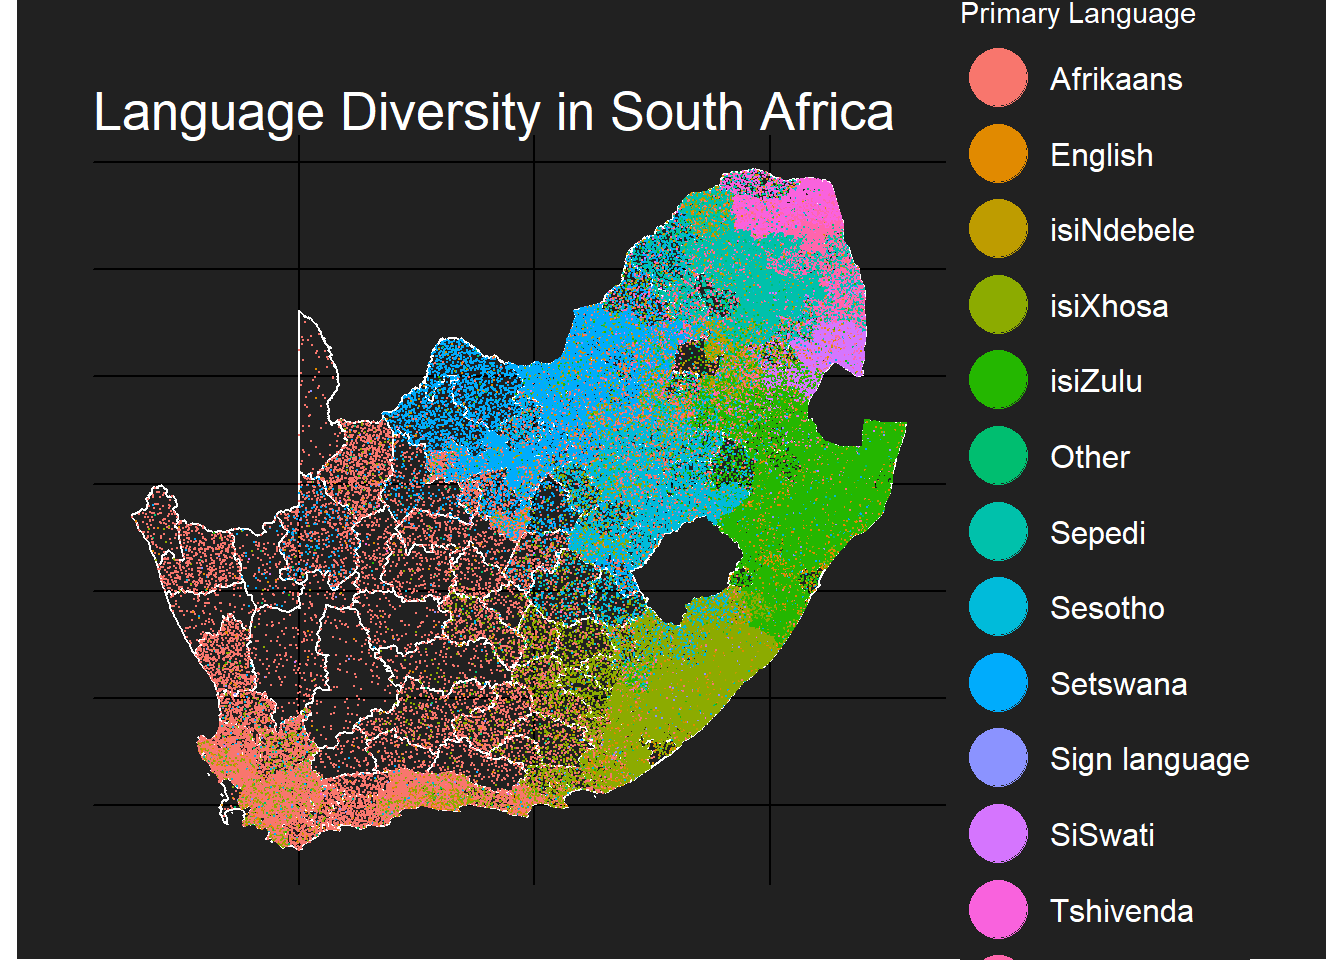
\includegraphics{2018-09-09-sf_chlorodot_files/figure-latex/plot_sa-1.pdf}

\begin{figure}
\centering
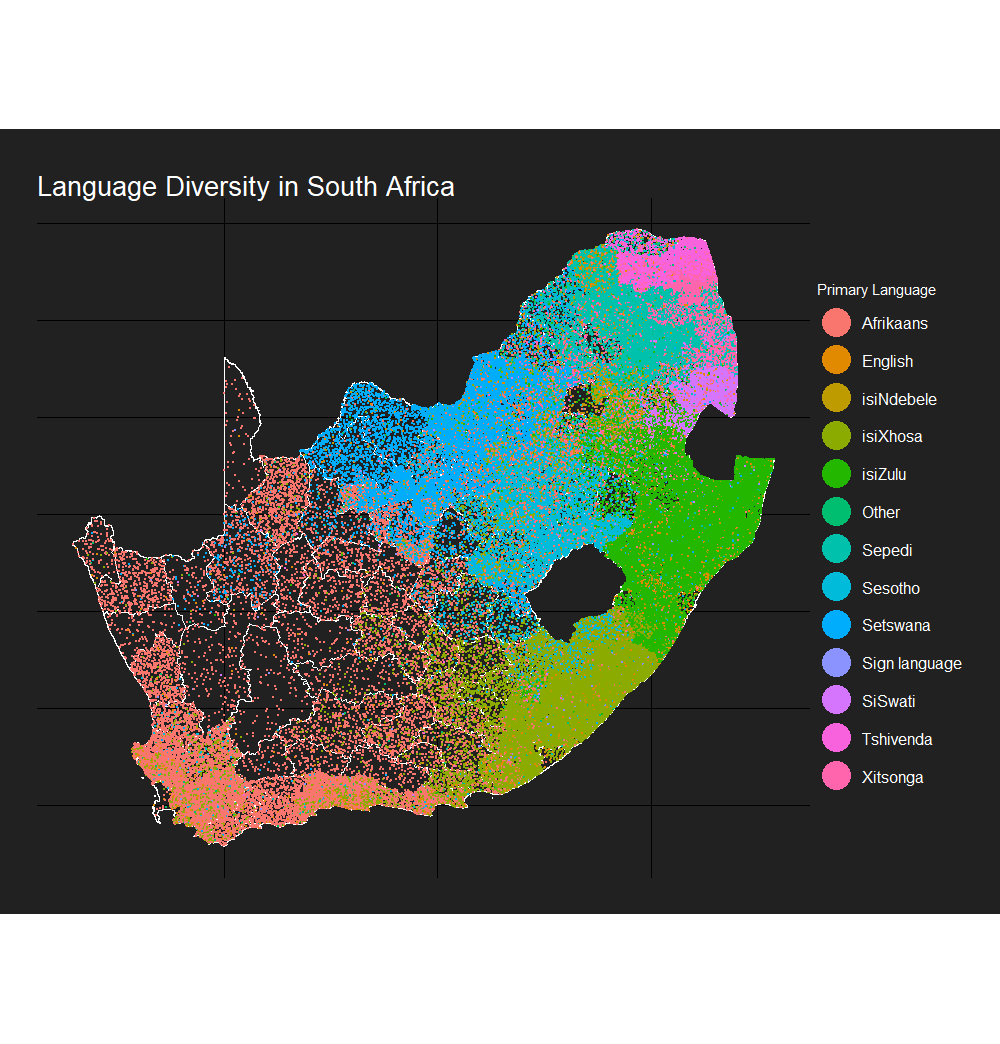
\includegraphics{C:/Users/Robert/Desktop/netlify_blog/static/img/south_africa.png}
\caption{South Africa}
\end{figure}

Enjoy!


\end{document}
